\documentclass{article}

\usepackage[fleqn]{amsmath}
\usepackage{amssymb}
\usepackage{hyperref}
\usepackage{url}
\usepackage{graphicx}
\usepackage{geometry}
\usepackage{babel}
\usepackage{enumitem}
\usepackage{parskip}
\usepackage{chemfig}
\usepackage{pdfpages}
\usepackage{xcolor}
\usepackage{tikz}
\usepackage{fancybox}
\usepackage{makecell}
\usepackage{pgfplots}
\usepackage{soul}
\usepackage{ulem}
\usepackage{wrapfig}
\usepackage{subcaption}
\usepackage[T1]{fontenc}
\usepackage{esvect}
\usetikzlibrary{arrows}
\usetikzlibrary{decorations.pathreplacing}
\pgfplotsset{compat=1.17}

\geometry{
    a4paper,
    total={170mm, 257mm},
    left=20mm,
    top=20mm
}

\hypersetup{
    colorlinks=true,
    linkcolor=black,
    urlcolor=blue,
    pdftitle={Context 1}
}

\newcommand{\figbox}[1]{ 
    \begin{figure*}[ht!]        
        \begin{center}            
            \fbox{#1}        
        \end{center}    
    \end{figure*}
}

\newcommand{\wrapfill}{
    \par
    \ifnum \value{WF@wrappedlines} > 0
        \addtocounter{WF@wrappedlines}{-1}%
        \null\vspace{
            \arabic{WF@wrappedlines}
            \baselineskip
        }
        \WFclear
    \fi
    \phantom{}
}

\newcommand{\cfig}[1]{%
  \begin{figure*}[ht!]%
    \centering%
    #1%
  \end{figure*}%
}

\newcommand{\difference}{\,\backslash\,}
\newcommand{\rem}{\underline{Remark}: }
\newcommand{\nots}{\underline{Notation}: }
\newcommand{\prf}{\underline{Proof}: }
\newcommand{\exs}{\underline{Example}: }
\newcommand{\defs}{\underline{Definition}: }
\newcommand{\wrn}{\underline{Warning}: }
\newcommand{\sht}{\ |\ }


% === TEXT ===
\title{\textbf{Context 1\\ HSLU, Semester 1}}
\author{Matteo Frongillo}

\begin{document}

\maketitle
\tableofcontents
\pagebreak

\section{Organigramm}
\hspace*{-1cm}
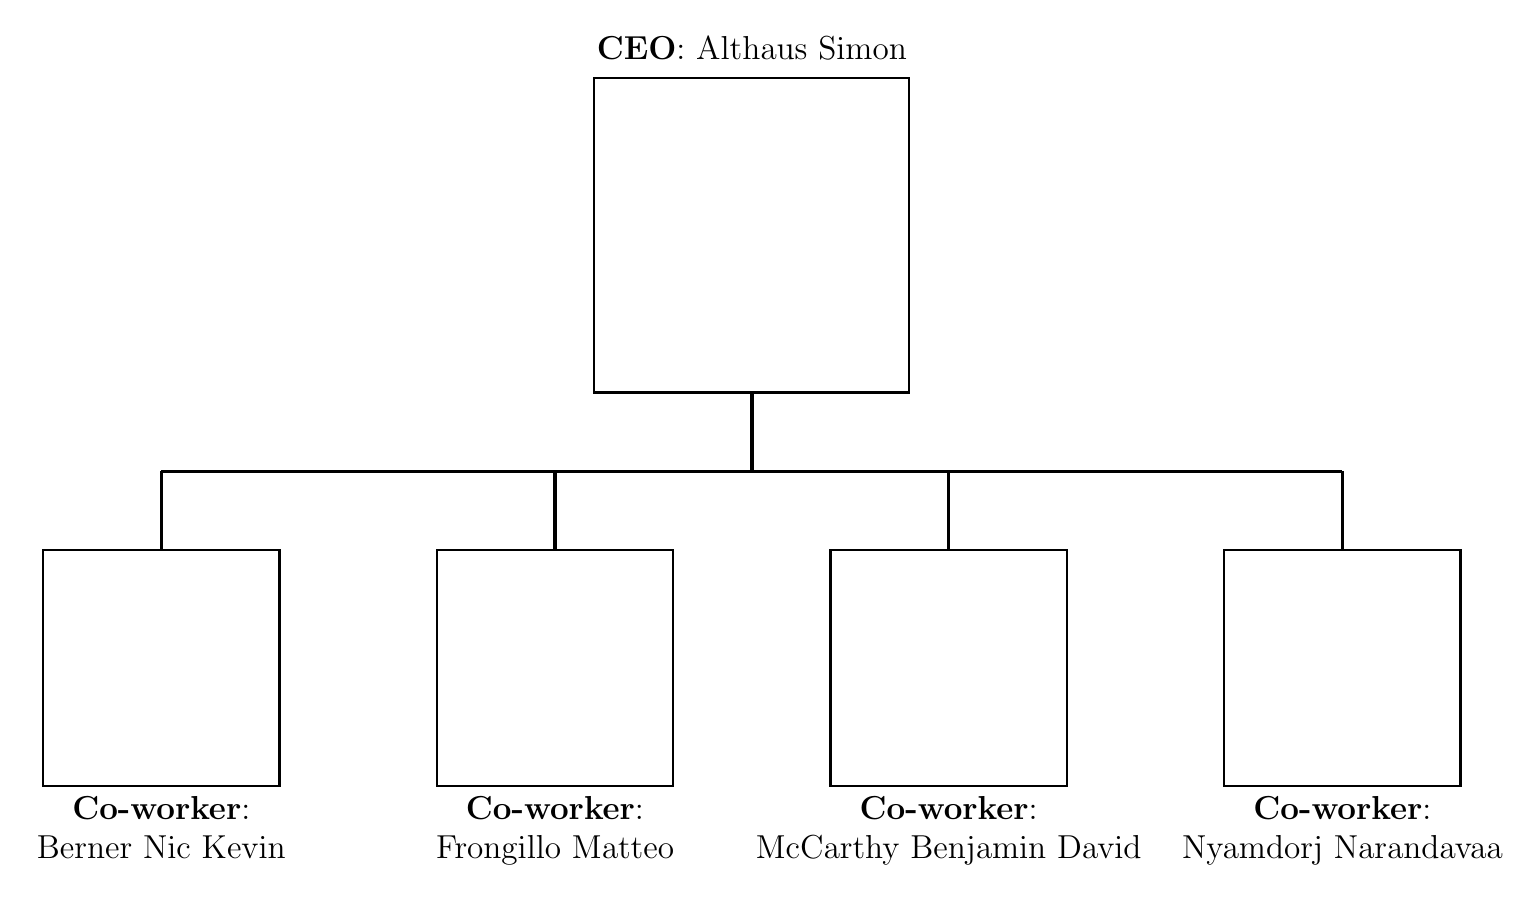
\begin{tikzpicture}
    \draw[thick] (-0.5,0) rectangle (3.5,4);
    \node[above] at (1.5,4.1) {\large \textbf{CEO}: Althaus Simon};

    \draw[very thick] (1.5,0) -- (1.5,-1);
    \draw[very thick] (-6,-1) -- (9,-1);

    \draw[very thick] (-6,-1) -- (-6,-2);
    \draw[very thick] (-1,-1) -- (-1,-2);
    \draw[very thick] (4,-1) -- (4,-2);
    \draw[very thick] (9,-1) -- (9,-2);

    \draw[thick] (-7.5,-2) rectangle (-4.5,-5);
    \node[below] at (-6,-5) {\large \textbf{Co-worker}:};
    \node[below] at (-6,-5.5) {\large Berner Nic Kevin};

    \draw[thick] (-2.5,-2) rectangle (0.5,-5);
    \node[below] at (-1,-5) {\large \textbf{Co-worker}:};
    \node[below] at (-1,-5.5) {\large Frongillo Matteo};

    \draw[thick] (2.5,-2) rectangle (5.5,-5);
    \node[below] at (4,-5) {\large \textbf{Co-worker}:};
    \node[below] at (4,-5.5) {\large McCarthy Benjamin David};

    \draw[thick] (7.5,-2) rectangle (10.5,-5);
    \node[below] at (9,-5) {\large \textbf{Co-worker}:};
    \node[below] at (9,-5.5) {\large Nyamdorj Narandavaa};

\end{tikzpicture}

\section{Meetings}
\begin{enumerate}
    \item Sunday 22.09.2024, 8pm
\end{enumerate}






\end{document}
